\documentclass[aspectratio=43]{beamer}
\usepackage{amsmath,amssymb,graphicx,listings,xcolor,booktabs}
\definecolor{aggiemaroon}{RGB}{80,0,0}
\setbeamercolor{structure}{fg=aggiemaroon}
\setbeamertemplate{navigation symbols}{}
\setbeamertemplate{footline}[frame number]
\setbeamertemplate{itemize items}[circle]
\lstdefinestyle{Rstyle}{language=R,basicstyle=\ttfamily\footnotesize,
  keywordstyle=\color{blue},commentstyle=\color{gray!70},
  stringstyle=\color{red!65!black},showstringspaces=false,
  breaklines=true,breakatwhitespace=true,columns=fullflexible,
  keepspaces=true,frame=single,framerule=0.25pt}
\lstset{style=Rstyle}

\title{Decision and Risk Analysis}
\subtitle{Lecture 8: \textbf{Posterior Inference \& Prediction}}
\author{}
\date{\color{aggiemaroon}{DAEN 427 / ISEN 427 / ISEN 627 - Fall 2026\\
      \textbf{Alexander Abuabara}}}
\titlegraphic{\vfill 
\includegraphics[height=1.2cm]{TAMU_logo.png}}

\begin{document}
\begin{frame}\titlepage\end{frame}

\begin{frame}{Learning objectives}
\begin{itemize}
\item Summarize a posterior with a point estimate\\and credible interval.
\item Evaluate hypotheses using posterior probabilities\\and Bayes factors.
\item Explain and compute posterior predictions for new obs.
\item Use MCMC draws to approximate\\and check posterior summaries.
\end{itemize}
\end{frame}

\begin{frame}{Our example: artists at MoMA}
\begin{itemize}
\item Let $\pi$ be the fraction of major modern-art museum artists born in 1965 or later.
\item In the MoMA sample, $Y=14$ of $n=100$ artists meet this definition.
\item Prior: $\pi\sim\mathrm{Beta}(4,6)$.
\item Sampling model: $Y\mid\pi\sim\mathrm{Bin}(100,\pi)$.
\end{itemize}
\[
\underbrace{\mathrm{Beta}(4,6)}_{\text{prior}}
\;\xrightarrow{\;Y=14\text{ of }100\;}\;
\underbrace{\mathrm{Beta}(18,92)}_{\text{posterior}}.
\]
\begin{block}{}
The data move our estimate toward 14\%,\\while the prior still contributes information.
\end{block}
\end{frame}

\begin{frame}[fragile]{R: inspect the sample and update}
\begin{lstlisting}
library(bayesrules)
library(tidyverse)
data("moma_sample")

moma_sample %>%
  group_by(genx) %>%
  tally()

plot_beta_binomial(alpha = 4, beta = 6,
                   y = 14, n = 100)
\end{lstlisting}
\end{frame}

\begin{frame}{}
\begin{itemize}
\item \texttt{bayesrules}: provides \texttt{moma\_sample} and plotting helpers.
\item \texttt{tidyverse}: \texttt{group\_by()}, \texttt{tally()}, and the \texttt{\%>\%} pipe.
\item \texttt{genx}: indicator for an artist born in 1965 or later.
\item \texttt{plot\_beta\_binomial()}: passes prior shapes $4,6$ and observed $y=14$, $n=100$.
\end{itemize}
\begin{block}{}
The posterior is concentrated near $0.16$\\and much narrower than the prior.
\end{block}
\end{frame}

\begin{frame}{Why is a point estimate not enough?}
\textbf{Question:} What percentage of artists are Gen X or younger?
\[
\begin{aligned}
E(\pi\mid Y=14)&=\frac{18}{110}\approx0.164,\\
\operatorname{Mode}(\pi\mid Y=14)&=\frac{17}{108}\approx0.157.
\end{aligned}
\]
\begin{itemize}
\item A typical posterior value is about 16\%.
\item But a point estimate hides uncertainty:
\begin{itemize}
\item $\mathrm{Beta}(18,92)$ vs. a wider $\mathrm{Beta}(4,16)$ posterior\\based on 10 observations. (check the book!)
\end{itemize}
\item Two analyses can have similar centers\\but very different precision.
\end{itemize}
\end{frame}

\begin{frame}{A 95\% posterior credible interval (CI)}
Let $f(\pi\mid y)$ be the posterior density, and $\pi_q$ its $q$th quantile.
\[
\text{Middle 95\% CI}=(\pi_{0.025},\pi_{0.975}),
\]
\[
P(\pi_{0.025}<\pi<\pi_{0.975}\mid Y=14)=0.95.
\]
For the posterior, the interval is approximately $(0.10,0.24)$.
\begin{block}{In plain-language ...}
Given the model and observed data, there is 95\% posterior probability that the population proportion is in this interval.
\end{block}
\end{frame}

\begin{frame}[fragile]{R}
\begin{lstlisting}
# Middle 95% credible interval
qbeta(c(0.025, 0.975), 18, 92)
# [1] 0.1009 0.2379

# Middle 50% credible interval
qbeta(c(0.25, 0.75), 18, 92)
# [1] 0.1388 0.1862

# Middle 99% credible interval
qbeta(c(0.005, 0.995), 18, 92)
# [1] 0.0853 0.2647
\end{lstlisting}
\end{frame}

\begin{frame}{}
\begin{itemize}
\item \texttt{qbeta()} is a \emph{base R} function: it returns Beta distribution quantiles.
\item First argument: quantile probabilities for the lower and upper endpoints.
\item Arguments \texttt{18, 92}: posterior Beta shape parameters.
\item The 50\% interval is narrowest; the 99\% interval is widest.
\end{itemize}
\begin{block}{Intuition}
Higher credibility requires including more posterior values, usually widening the interval. Highest-density intervals are an alternative to equal-tailed intervals.
\end{block}
\end{frame}

\begin{frame}{\textbf{Posterior hypothesis testing}\\One-sided question: is $\pi<0.20$?}
\[
H_0:\pi\ge0.20\qquad H_a:\pi<0.20.
\]
The probability of the claim is an area under the posterior density:
\[
P(H_a\mid Y=14)=\int_0^{0.20}f(\pi\mid Y=14)\,d\pi
=0.849.
\]
\begin{block}{}
Given the prior, sampling model, and 100 observed artists,\\the posterior chance that the population proportion is below 20\% is about 84.9\%.
\end{block}
\end{frame}

\begin{frame}[fragile]{R (probability, odds, and Bayes factor)}
\begin{lstlisting}
post_prob <- pbeta(0.20, 18, 92)
post_odds <- post_prob / (1 - post_prob)

prior_prob <- pbeta(0.20, 4, 6)
prior_odds <- prior_prob / (1 - prior_prob)
BF <- post_odds / prior_odds

post_prob  # 0.849
post_odds  # 5.622
prior_prob # 0.08564
prior_odds # 0.09366
BF         # 60.02
\end{lstlisting}
\end{frame}

\begin{frame}{}
\begin{itemize}
\item \texttt{pbeta(x,a,b)} (base R): $P(\pi\le x)$ for a $\mathrm{Beta}(a,b)$ variable.
\item \texttt{post\_odds}: probability of $H_a$ divided by probability of $H_0$ after observing data.
\item \texttt{prior\_odds}: the same ratio before observing data.
\item \texttt{BF}: posterior odds divided by prior odds.
\end{itemize}
\[
\mathrm{BF}=\frac{P(H_a\mid y)/P(H_0\mid y)}
{P(H_a)/P(H_0)}\approx60.
\]
\begin{block}{Intuition}
The sample multiplies the odds for $\pi<0.20$ by about 60;\\a Bayes factor is not itself a probability.
\end{block}
\end{frame}

\begin{frame}{What about a two-sided claim?}
\textbf{Question:} Is the true proportion different from $0.30$?
\[
H_0:\pi=0.30\qquad H_a:\pi\ne0.30.
\]

\begin{itemize}
\item Under the continuous Beta prior and posterior, $P(\pi=0.30)=0$.
\item So the previous odds-ratio calculation cannot test this exact point null.
\item The 95\% CI $(0.10,0.24)$ lies below $0.30$.
\item Chapter 8 suggests a specified meaningful range: $H_0:\pi\in(0.25,0.35)$.
\end{itemize}
\begin{block}{Note}
Define what counts as a meaningful difference \emph{before} examining the data.
(a point-mass prior would be a different model)
\end{block}
\end{frame}

\begin{frame}{\textbf{Posterior prediction}\\Predict 20 new artworks}
Let $Y'$ count younger artists in 20 \emph{new} artworks.
\[
Y'\mid\pi\sim\mathrm{Bin}(20,\pi),\quad
P(Y'=y'\mid\pi)={20\choose y'}\pi^{y'}(1-\pi)^{20-y'}.
\]
\begin{itemize}
\item Even for a known $\pi$, the new count varies by random sampling.
\item We are also uncertain about $\pi$ itself.
\end{itemize}
\begin{block}{Intuition}
Prediction must account for both sampling variability \emph{and} posterior uncertainty about the rate.
\end{block}
\end{frame}
\begin{frame}{Posterior predictive distribution}
Average new-data probabilities over plausible parameter values:
\[
f(y'\mid y)=\int_0^1 f(y'\mid\pi)f(\pi\mid y)\,d\pi.
\]
Here $y=14$ and $\pi\mid y\sim\mathrm{Beta}(18,92)$.
\begin{itemize}
\item Exact predictive probability: $P(Y'=3\mid Y=14)=0.2217$.
\item $P(Y'\ge5\mid Y=14)=0.233$.
\item $E(Y'\mid Y=14)=3.273$; the most likely count is 3.
\end{itemize}
\begin{block}{Meaning}
Three is the best single-count prediction, not a guarantee.
\end{block}
\end{frame}

\begin{frame}[fragile]{Calculate predictive probabilities}
\begin{lstlisting}
# Beta-binomial predictive probabilities;
# base R's beta and choose functions
ys <- 0:20
pred <- choose(20, ys) *
  beta(18 + ys, 92 + 20 - ys) /
  beta(18, 92)

pred[ys == 3]           # about 0.2217
sum(pred[ys >= 5])      # about 0.233
sum(ys * pred)          # about 3.273
\end{lstlisting}
\footnotesize This is an R implementation;\\the book displays the analytic calculation rather than this code.
\end{frame}
\begin{frame}{Exact prediction}
\begin{itemize}
\item \texttt{ys <- 0:20}: enumerate all possible counts in the next 20 observations.
\item \texttt{choose(20, ys)}: count ways each outcome can occur.
\item \texttt{beta()} (base R): evaluates the Beta function; its ratio averages over the posterior for $\pi$.
\item \texttt{pred}: probability of each count; it sums to 1.
\item \texttt{sum()} and indexing: add probabilities for $Y'\ge5$, or calculate a weighted average.
\end{itemize}
\begin{block}{Intuition}
The predictive distribution spreads probability across many possible future counts, not only 3.
\end{block}
\end{frame}

\section{8.4 Posterior analysis with MCMC}
\begin{frame}{When exact calculations are unavailable}
\textbf{Question:} Can a sample of plausible $\pi$ values replace difficult integrals?
\begin{itemize}
\item MCMC generates dependent draws that approximate the posterior distribution.
\item Chapter 8 uses four chains with 10,000 iterations each and discards the first 5,000 of each.
\item That leaves $4\times5{,}000=20{,}000$ posterior draws.
\item Check simulation quality \emph{before} interpreting summaries.
\end{itemize}
\begin{block}{Intuition}
A posterior probability can be approximated by the fraction of simulated draws satisfying a claim.
\end{block}
\end{frame}
\begin{frame}[fragile]{Specify and simulate the model}
\begin{lstlisting}
library(rstan)
art_model <- "
data { int<lower=0,upper=100> Y; }
parameters { real<lower=0,upper=1> pi; }
model {
  Y ~ binomial(100, pi);
  pi ~ beta(4, 6);
}"

art_sim <- stan(model_code = art_model,
                data = list(Y = 14),
                chains = 4, iter = 10000,
                seed = 84735)
\end{lstlisting}
\end{frame}

\begin{frame}{Explaining Stan}
\begin{itemize}
\item \texttt{rstan} interfaces R with Stan's posterior simulation engine.
\item \texttt{data}: $Y$ is the observed count, constrained between 0 and 100.
\item \texttt{parameters}: unknown proportion $\pi$ is constrained to $[0,1]$.
\item \texttt{model}: binomial sampling model plus Beta prior.
\item \texttt{stan()}: simulates four chains, each of length 10,000; default warmup discards half.
\end{itemize}
\begin{block}{Expected result}
A fitted \texttt{stanfit} object containing 20,000 retained draws across four chains. Actual draw values depend on the software environment.
\end{block}
\end{frame}

\begin{frame}[fragile]{MCMC Diagnostics}
\begin{lstlisting}
library(bayesplot)

mcmc_trace(art_sim, pars = "pi")
mcmc_dens_overlay(art_sim, pars = "pi")
mcmc_acf(art_sim, pars = "pi")

rhat(art_sim, pars = "pi")
neff_ratio(art_sim, pars = "pi")
\end{lstlisting}
\small Reported diagnostics: \texttt{Rhat = 1}; \texttt{neff\_ratio = 0.378}.\par
\small Expected plots: well-mixed traces, overlapping chain densities,\\and quickly decaying autocorrelation (see Fig.~8.8).
\end{frame}

\begin{frame}{}
\small
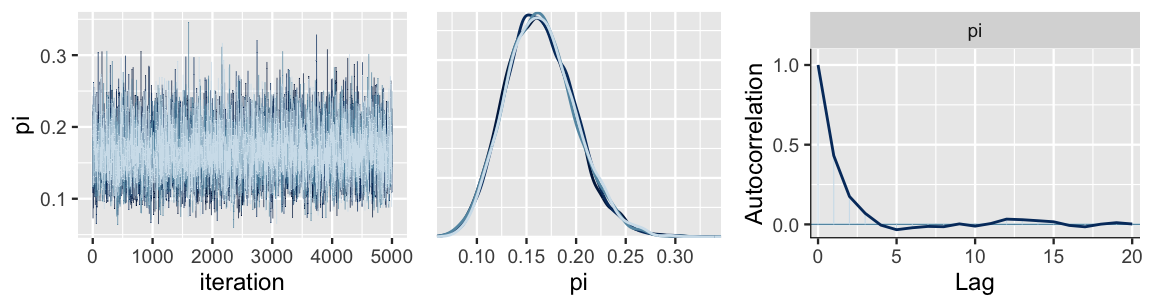
\includegraphics[width=.95\textwidth]{art-sim-1-ch8-1.png}
\begin{itemize}
    \setlength{\itemsep}{0.1cm}
    \item \textbf{Trace plot:}
    The chains fluctuate around a stable value,
    with no obvious trends or prolonged periods of
    getting stuck.
    \item \textbf{Posterior density:}
    The chains produce similar posterior distributions,
    centered around $\pi \approx 0.16$.

    \item \textbf{Autocorrelation:}
    The dependence between successive samples
    decreases quickly and approaches zero
    after approximately 5 lags.

\end{itemize}

\vspace{0.1cm}

The rapid decrease in autocorrelation suggests
\textbf{relatively good mixing}: the chain explores
the posterior efficiently rather than remaining
stuck in the same region for long periods.
\end{frame}

\begin{frame}{Diagnostics}
\begin{itemize}
\item \texttt{bayesplot}: trace, density overlay, and autocorrelation graphics.
\item \texttt{rhat()}: checks consistency across chains; near 1 is desirable.
\item \texttt{neff\_ratio()}: effective sample size divided by retained sample size.
\item The ratio $0.378$ corresponds to approximately 7,600 independent-equivalent draws.
\end{itemize}
\begin{block}{Intuition}
20,000 correlated MCMC draws are not necessarily as informative as 20,000 independent draws. Recheck diagnostics for your own run.
\end{block}
\end{frame}

\begin{frame}[fragile]{Summarize the MCMC posterior}
\begin{lstlisting}
library(broom.mixed)
library(janitor)

tidy(art_sim, conf.int = TRUE,
     conf.level = 0.95)

art_chains_df <- as.data.frame(
  art_sim, pars = "pi")

mean(art_chains_df$pi)
quantile(art_chains_df$pi, c(0.025, 0.975))
mean(art_chains_df$pi < 0.20)
\end{lstlisting}
\small Output from \texttt{tidy()}: median $0.162$, CI $(0.101,0.239)$.\par
\small MCMC estimate of $P(\pi<0.20\mid y)$: $0.846$.
\end{frame}

\begin{frame}{Simulated inference}
\begin{itemize}
\item \texttt{broom.mixed::tidy()}: posterior median, uncertainty summaries, and central 95\% interval for the fitted parameter.
\item \texttt{as.data.frame()}: combine retained chain draws of $\pi$ into an R table.
\item \texttt{mean()} and \texttt{quantile()}: approximate posterior center and interval endpoints.
\item \texttt{mean(pi < 0.20)}: fraction of draws consistent with the claim.
\item \texttt{janitor} is used for the "optional" \texttt{tabyl()} count table;\\it is not required for these shortened lines.
\end{itemize}
\begin{block}{}
MCMC approximates the exact 95\% CI $(0.1009,0.2379)$ and exact posterior probability $0.849$.
\end{block}
\end{frame}

\begin{frame}[fragile]{Simulate and summarize predictions}
\begin{lstlisting}
set.seed(1)
art_chains_df <- art_chains_df %>%
  mutate(y_predict = rbinom(
    length(pi), size = 20, prob = pi))

ggplot(art_chains_df,
       aes(x = y_predict)) + stat_count()

art_chains_df %>%
  summarize(mean = mean(y_predict),
    lower_80 = quantile(y_predict, 0.10),
    upper_80 = quantile(y_predict, 0.90))
\end{lstlisting}
\small Output: mean $3.283$, central 80\% interval from 1 to 6.
\end{frame}

\begin{frame}
\center 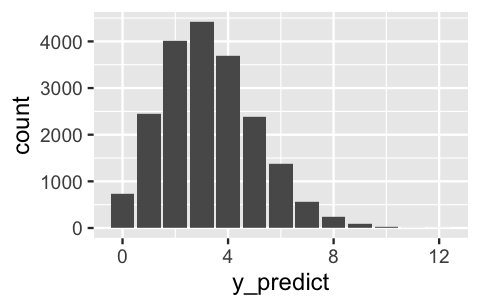
\includegraphics[width=.6\textwidth]{ch8-hist-1.png}
\begin{itemize}
\item A histogram of 20,000 simulated posterior predictions of the number among the next 20 artists that will be Gen X or younger.
\item We expect roughly 3 of the next 20 artists to be Gen X or younger, but there’s an 80\% chance that this figure is somewhere between 1 and 6 artists.
\end{itemize}
\end{frame}

\begin{frame}{Explaining the code: predictive simulation}
\begin{itemize}
\item \texttt{set.seed(1)}: makes the R random-number stream reproducible.
\item \texttt{rbinom()}: for \emph{each} simulated $\pi$, draws a new count out of 20.
\item \texttt{mutate()}: adds these counts as \texttt{y\_predict}.
\item \texttt{ggplot() + stat\_count()}: plots the frequency of each predicted count.
\item \texttt{summarize()} and \texttt{quantile()}: predictive mean and middle 80\% endpoints.
\end{itemize}
\begin{block}{Meaning ...}
Given the model and data, the simulation places about 80\% of predicted 20-artwork counts between 1 and 6.
\end{block}
\end{frame}

\begin{frame}{\textbf{Bayesian benefits}\\Conditioning matters: posterior vs. $p$-value}
Two probabilities in the chapter answer \emph{different} questions:
\[
\underbrace{P(\pi<0.20\mid Y=14)=0.849}_{\text{uncertainty about a parameter given data}}
\]
\[
\underbrace{P(Y\le14\mid\pi=0.20)=0.08}_{\text{data variability under an assumed rate}}
\]
\begin{block}{Intuition}
The second quantity does not say there is an 8\% chance that the assumed parameter value is true.
Neither quantity is a universal true/false decision rule.
\end{block}
\end{frame}
\begin{frame}{Key takeaways}
\begin{enumerate}
\item \textbf{Estimation:} report both a posterior center and uncertainty interval.
\item \textbf{Testing:} posterior probability assesses a claim; a Bayes factor compares changes in odds.
\item \textbf{Prediction:} average over uncertain parameters and future sampling randomness.
\item \textbf{MCMC:} approximate all three tasks from posterior draws, after checking diagnostics.
\end{enumerate}
\end{frame}

\begin{frame}{Check your understanding}
\small
\begin{enumerate}
\item \textbf{Is a 95\% credible interval a 95\% range for a new count?}\\
\item[] 
\item \textbf{Does a Bayes factor of 60 mean $P(H_a\mid y)=0.60$?}\\
\item[]
\item \textbf{Why not always predict exactly 3 new younger artists?}\\
\item[]
\item \textbf{Do many MCMC draws guarantee correct results?}\\
\item[]
\end{enumerate}
\end{frame}

\begin{frame}{Check your understanding (short answers here)}
\small
\begin{enumerate}
\item \textbf{Is a 95\% credible interval a 95\% range for a new count?}\\
\textcolor{blue}{No. It describes $\pi$, not the future count $Y'$.}
\item \textbf{Does a Bayes factor of 60 mean $P(H_a\mid y)=0.60$?}\\
\textcolor{blue}{No. It is the ratio of posterior odds to prior odds.}
\item \textbf{Why not always predict exactly 3 new younger artists?}\\
\textcolor{blue}{Both the future sample and $\pi$ vary.}
\item \textbf{Do many MCMC draws guarantee correct results?}\\
\textcolor{blue}{No. Convergence and mixing must be assessed.}
\end{enumerate}
\end{frame}

\end{document}